%%%%%%%%%%%%%%%%%%%%%%%%%%%%%%%%%%%%%%%%%%%%%%%%%%%%%%%%%%%%%%%%%%%%%%%%
\chapter{Introduction}
\label{chapter:ch1-introduction}
%%%%%%%%%%%%%%%%%%%%%%%%%%%%%%%%%%%%%%%%%%%%%%%%%%%%%%%%%%%%%%%%%%%%%%%%
\localtoc

%%%%%%%%%%%%%%%%%%%%%%%%%%%%%%%%%%%%%%%%%%%%%%%%%%%%%%%%%%%%%%%%%%%%%%%%%%%%%%%
\section{Context and Motivation}
\label{section:ch1-context_and_motivation}
%%%%%%%%%%%%%%%%%%%%%%%%%%%%%%%%%%%%%%%%%%%%%%%%%%%%%%%%%%%%%%%%%%%%%%%%%%%%%%%

\begin{figure}[t]
  \centering
  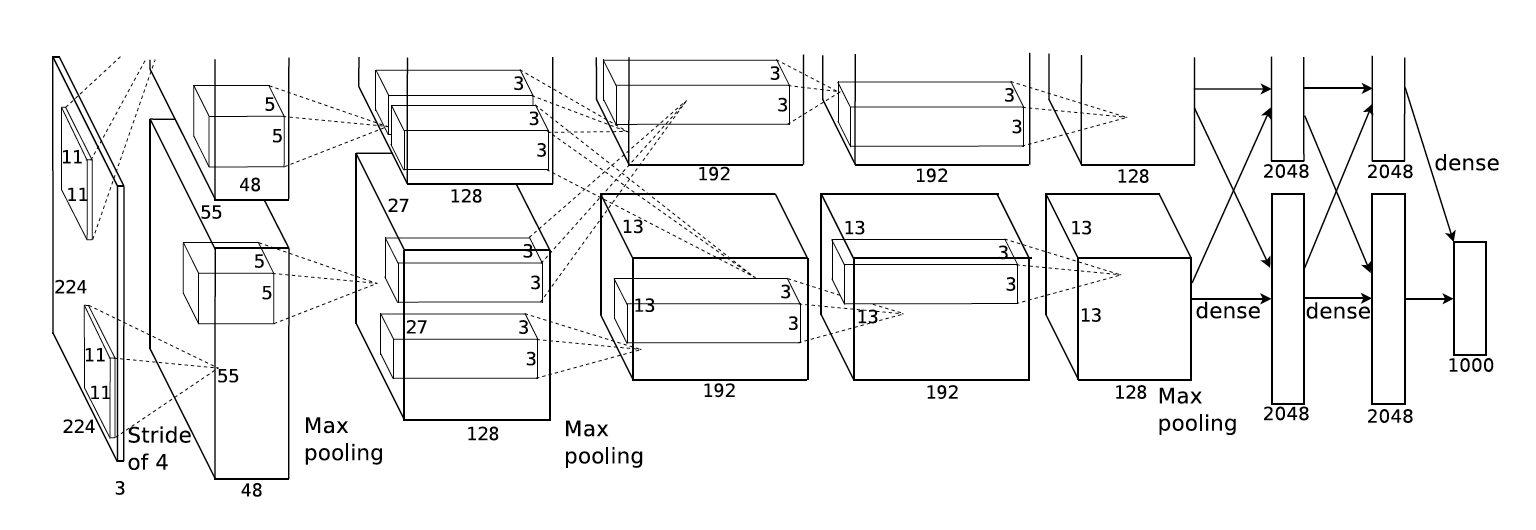
\includegraphics[scale=0.2]{figures/main/ch1-introduction/alexnet.png}
  \caption{The neural network architecture (AlexNet) proposed by~\citet{krizhevsky2012imagenet} which won the ImageNet Large-Scale Visual Recognition Challenge in 2012.}
  \label{figure:ch1-alexnet_network}
\end{figure}

One of the most remarkable breakthroughs of Deep Learning happened in 2012 during the ImageNet Large-Scale Visual Recognition Challenge~\cite{russakovsky2015imagenet}.
The challenge aims at evaluating different algorithms for object detection and image classification.
In 2012, \citeauthor{krizhevsky2012imagenet} obtained \nth{1} place and beat every other participant by a 10.8\% margin with a neural network architecture called \textbf{AlexNet}.
The main reasons for this success are twofold.
First, they used a convolutional neural network (CNN) with more than 60 million parameters which was one of the largest models of the time.
Secondly, they designed a specific architecture to exploit dual programmable graphics processing units (GPUs) to speed up the arithmetic operations, which enabled them to significantly reduce training time.
The \Cref{figure:ch1-alexnet_network} shows the AlexNet architecture which consists of five convolutional layers with two fully connected layers at the end.
The figure also shows the distribution of the workload between the two GPUs.


\begin{table}[t]
  \centering
  \sisetup{
    table-number-alignment = center,
    table-space-text-pre = \ \ \ ,
  }
  \begin{subfigure}[b]{\textwidth}
    \centering
    \begin{tabular}{
      L{5cm}
      L{3.5cm}
      S[table-format=3.0, table-text-alignment=left]@{\,}
      s[table-unit-alignment=left]
      c
    }
      \toprule
      \textbf{Authors} & \textbf{Models} & \multicolumn{2}{c}{\textbf{\#Params}} & \textbf{TOP-5 Acc.} \\
      \midrule
      \citet{krizhevsky2012imagenet} & AlexNet             &  61 & \si{M} & 84.7\% \\
      \citet{simonyan2014very}       & VGG                 & 144 & \si{M} & 92.0\% \\
      \citet{he2016deep}             & ResNet-152          &  60 & \si{M} & 93.8\% \\
      \citet{szegedy2017inception}   & Inception-ResNet-v2 &  56 & \si{M} & 95.1\% \\
      \citet{xie2017aggregated}      & ResNeXt-101         &  84 & \si{M} & 95.6\% \\
      \citet{hu2018squeeze}          & SENet               & 146 & \si{M} & 96.2\% \\
      \citet{real2019regularized}    & AmoebaNet-A         & 469 & \si{M} & 96.7\% \\
      \citet{huang2019gpipe}         & AmoebaNet-B         & 556 & \si{M} & 97.0\% \\
      \bottomrule
    \end{tabular}
    \caption{Computer Vision Models}
    \label{table:ch1-networks_parameters_cv}
  \end{subfigure}
  \par\bigskip
  \begin{subfigure}[b]{\textwidth}
    \centering
    \begin{tabular}{
      L{4.5cm}
      L{4.5cm}
      S[table-format=3.0, table-text-alignment=left]@{\,}
      s[table-unit-alignment=left]
    }
      \toprule
      \textbf{Authors} & \textbf{Models} & \multicolumn{2}{c}{\textbf{\#Params}} \\
      \midrule
      \citet{peters2018deep}         & ELMo            &  94 & \si{M} \\
      \citet{radford2018improving}   & GPT             & 110 & \si{M} \\
      \citet{devlin2019bert}         & BERT            & 340 & \si{M} \\
      \citet{yang2019xlnet}          & XLNet (Large)   & 340 & \si{M} \\
      \citet{liu2019roberta}         & RoBERTa (Large) & 355 & \si{M} \\
      \citet{radford2019language}    & GPT-2           &   1 & \si{B} \\
      \citet{shoeybi2019megatron}    & MegatronLM      &   8 & \si{B} \\
      \citet{raffel2020exploring}    & T5-11B          &  11 & \si{B} \\
      \citet{rosset2020turingnlg}    & T-NLG           &  17 & \si{B} \\
      \citet{brown2020language}      & GPT-3           & 175 & \si{B} \\
      \citet{fedus2021switch}        & Switch Transformers & 1 & \si{T} \\
      \bottomrule
    \end{tabular}
    \caption{Natural Language Processing Models}
    \label{table:ch1-networks_parameters_nlp}
  \end{subfigure}
  \par\bigskip
  \caption{Evolution of the number of parameters for Computer Vision and Natural Language Processing models developed in the years after AlexNet.}
  %   List of Computer Vision and Natural Language Processing models with their number of param
  %   Tables showing the different network architectures developed in the years after AlexNet.
  %   \Cref{table:ch1-networks_parameters_cv} shows networks developed for computer vision tasks and \Cref{table:ch1-networks_parameters_nlp} shows networks developed for natural language processing.
  % }
  \label{table:ch1-networks_parameters}
\end{table}


Following this result, many architectures with an increasing number of parameters have been developed.
This growth in the number of parameters has led to an increase in accuracy, exceeding even human performance, on the ImageNet dataset~\cite{he2015delving}.
\Cref{table:ch1-networks_parameters} shows a list of the different state-of-the-art architectures along with their size and accuracy.
As we can see, the accuracy of the models generally improves at the cost of the model size.
For computer vision models, \citet{tan2019efficientnet} have shown that the relationship between model size and accuracy seems to obey a power law.
% This relationship has also been observed for Natural Language Processing (NLP) neural networks \cite{rosenfeld2020a,kaplan2020scaling} and given the availability of large-scale datasets (Common Crawl dataset~\cite{raffel2020exploring} constitutes nearly a trillion words), researchers have been able to scale their models.
This relationship has also been observed for Natural Language Processing (NLP) neural networks \cite{rosenfeld2020a,kaplan2020scaling} aided by the availability of large-scale datasets such as the Common Crawl dataset~\cite{raffel2020exploring} which constitutes nearly a trillion words.

As a result of their size and improved accuracy, deep neural networks now achieve state-of-the-art performances in a variety of domains such as image recognition~\cite{lecun1998gradient,krizhevsky2012imagenet,he2016deep,tan2019efficientnet}, object detection~\cite{redmon2016you,liu2016ssd,redmon2017yolo9000}, natural language processing~\cite{merity2016pointer,vaswani2017attention,radford2019language,brown2020language}, speech recognition~\cite{hinton2012deep,abdel2014convolutional,yu2016automatic}, health care \cite{faust2018deep} etc.
Specifically, computer vision and natural language processing models have achieved sufficient performance for being used in real-world applications such as autonomous vehicles~\cite{fagnant2015preparing,sharma2021automating}, translation~\cite{wu2016google}, vocal assistants~\cite{li2017acoustic}, etc.

However, accuracy is not the only concern, when implemented in a critical decision process, neural networks need to be compact, cost-effective and secure.
Although accurate, large neural networks often lack these properties.
Indeed, training state-of-the-art models on computer vision or natural language processing tasks requires gigabytes of memory and can take several months on a single GPU~\cite{krizhevsky2012imagenet,brown2020language}.
For example, the GPT-3 model proposed by~\citet{brown2020language}, culminates at 175 billion parameters and requires 355 years of training on a single GPU and \$\numprint{4600000} to train on a cloud-computing platform \cite{li2020overview}.
It has also been estimated by \citet{strubell2019energy} that the training and development costs of the large Transformer model proposed by~\citet{vaswani2017attention} with neural architecture search emits an estimated \numprint{284019} kg of $\mathrm{CO}_2$ whereas a human life will consume an average of \numprint{5000} kg of $\mathrm{CO}_2$ for one year. 
Furthermore, with the rise of smartphones and ``Internet of things'' devices (IoT) with limited computational and memory resources, neural networks also need to be efficient during the inference phase.
In addition, with the growing concern over data privacy, methods such as \emph{federated learning} are gaining ground.
Federated learning involves training a model across multiple decentralized devices (\eg, smartphones) with local data samples.
This avoids the step of centralizing all users' data into one server, thus addressing the issue of data privacy.
Thus, building compact and cost-effective neural networks have been an important goal in order to reduce training time, reduce cost and allow for faster research and development.

In addition to being compact and cost-effective, neural networks also need to be secure.
Due to a high complexity and expressivity, large neural networks exhibit instability to small perturbations of their inputs.
Unstable neural networks tend to be vulnerable to \emph{adversarial examples}, \ie, imperceptible variations of natural examples, crafted to deliberately mislead the models~\cite{globerson2006nightmare,biggio2013evasion,szegedy2013intriguing}.
The \Cref{figure:ch1-adversarial_image_example} gives an example of an adversarial attack on an image.
The small perturbation (center) is added to the original image (left) leading to an adversarial image (right).
This behavior can cause serious security problems when neural networks are used for critical decision-making (\eg, judicial decision, self-driving cars, etc.).

This thesis focuses on the problem of training neural networks which are not only accurate but also compact, easy to train, reliable and robust to adversarial examples.





% The study of security properties of learning algorithms is a research field known as \emph{adversarial machine learning} which dates back to 2004 \cite{dalvi2004adversarial}.
% More recently, the work of \citet{szegedy2013intriguing} has brought considerable attention to adversarial examples in the context of Deep Learning.
% Since then, a number of work has been published in designing attacks and defenses \cite{szegedy2013intriguing,goodfellow2014explaining,papernot2016limitations,madry2018towards,carlini2017towards,pinot2019theoretical}.
% \emph{Adversarial Training} (AT), one of the first effective methods to protect against adversarial examples, was introduced by \citet{goodfellow2014explaining} and later improved by \citet{madry2018towards}.
% It consists of augmenting training batches with adversarial examples generated during the training procedure.
% More recently, a new method \cite{farnia2018generalizable} based on the regularization of the Lipschitz constant of the network has been proposed which linked the generalization capabilities of neural networks to their Lipschitz constant; therefore, a reduced Lipschitz constant could lead to a better generalization.
% Although these methods improve the robustness of neural networks, the accuracy obtained ``under attack'' is far from state-of-the-art and therefore security risks are still present.
%






%%%%%%%%%%%%%%%%%%%%%%%%%%%%%%%%%%%%%%%%%%%%%%%%%%%%%%%%%%%%%%%%%%%%%%%%%%%%%%%
\section{Problem Statement and Contributions}
\label{section:ch1-problem_statement_and_contributions}
%%%%%%%%%%%%%%%%%%%%%%%%%%%%%%%%%%%%%%%%%%%%%%%%%%%%%%%%%%%%%%%%%%%%%%%%%%%%%%%


\begin{figure}[t]
   \centering
   \begin{subfigure}[t]{0.24\textwidth}
       \centering
       \begin{equation*}
	  \leftmatrix
	    a &   &   &   \\
	      & b &   &   \\
	      &   & c &   \\
	      &   &   & d
	  \rightmatrix
       \end{equation*}
       \caption*{diagonal}
   \end{subfigure}
   \hfill
   \begin{subfigure}[t]{0.24\textwidth}
       \centering
       \begin{equation*}
	  \leftmatrix
	    a & b & c & d \\
	    e & a & b & c \\
	    f & e & a & b \\
	    d & f & e & a
	  \rightmatrix
       \end{equation*}
       \caption*{Toeplitz}
   \end{subfigure}
   \hfill
   \begin{subfigure}[t]{0.24\textwidth}
       \centering
       \begin{equation*}
	  \leftmatrix
	    ae & af & ag & ah \\
	    be & bf & bg & bh \\
	    ce & cf & cg & ch \\
	    de & df & dg & dh
	  \rightmatrix
       \end{equation*}
       \caption*{Low Rank}
   \end{subfigure}
   \hfill
   \begin{subfigure}[t]{0.24\textwidth}
       \centering
       \begin{equation*}
	  \leftmatrix
	    a & a^2 & a^3 & a^4 \\
	    b & b^2 & b^3 & b^4 \\
	    c & c^2 & c^3 & c^4 \\
	    d & d^2 & d^3 & d^4
	  \rightmatrix
       \end{equation*}
       \caption*{Vandermonde}
   \end{subfigure}
  \caption{Examples of structured matrices.}
  \label{figure:ch1-example_structure_matrices}
\end{figure}


Neural networks, which find their roots in the work of \citet{mcculloch1943logical,rosenblatt1958perceptron}, can be analytically described as a composition of multi-dimensional linear functions interlaced with nonlinear functions (also called activation functions).
More formally, a neural network is a function $N_{\Omega} : \Rbb^n \rightarrow \Rbb^m$ parameterized by a set of weights $\Omega$ of the form:
\begin{equation} \label{equation:ch1-neural_network}
  N_{\Omega}(\xvec) = \psi^{(\depth)} \circ \rho \circ \psi^{(\depth-1)} \cdots \circ \psi^{(2)} \circ \rho \circ \psi^{(1)} (\xvec) \enspace.
\end{equation}
Here, $\depth$ corresponds to the \emph{depth} of the network (\ie, the number of layers) and $\rho$ is a nonlinear function.
Finally, each $\psi^{(i)}$ is a multi-dimensional linear function $\psi^{(i)}: \xvec \mapsto \Wmat^{(i)} \xvec + \bvec^{(i)}$ parameterized by a weight matrix $\Wmat^{(i)}$ and a bias vector $\bvec^{(i)}$ and $\Omega$ is the union of the parameters of each layer. 
% (we present a more formal definition of neural networks in~\Cref{chapter:ch2-background}). 


Classical neural networks typically have a large number of parameters to train.
% For example, a two-layer \emph{fully connected neural networks}, networks in which all the neurons from one activation are connected to all the neurons of the following activation -- \ie, meaning the weight matrix of each layer is \emph{dense} -- will have a minimum of $n \times m + m^2$ parameters where $n$ is the size of the input and $m$ is the size of the output (number of classes).
% The dimension of the input is usually large, for example, with the ImageNet dataset $n = 224^2 \times 3$ and $m = 1000$ leading to a two-layer fully connected neural network with more than 150 million parameters.
If they have no restrictions on the weight matrices $\Wmat^{(i)}$, the layers are said to be \emph{fully connected}.
Typically, fully connected neural networks have a large number of parameters.
For example, a fully connected neural network with $\depth$ layers and $n$ neurons on each layer ($\Wmat^{(i)} \in \Rbb^{n \times n}$) will have $\bigO\left(pn (n + 1)\right)$ parameters.
Since the input and output dimensions are generally large (\eg, ImageNet has an input dimension of $224^2 \times 3$ and an output of 1000), simple fully connected neural networks with few layers accumulate over hundreds of millions of parameters.
Generally, this type of neural network has been shown to perform poorly due to a large search space.
Moreover, they are computationally expensive, which makes them impractical for a number of use cases (smartphones, IoT devices, etc.).
To reduce the number of parameters on each layer, researchers have devised specific linear operations that reduce the number of parameters and have better properties for the problem at hand.


\begin{figure}[t]
  \centering
  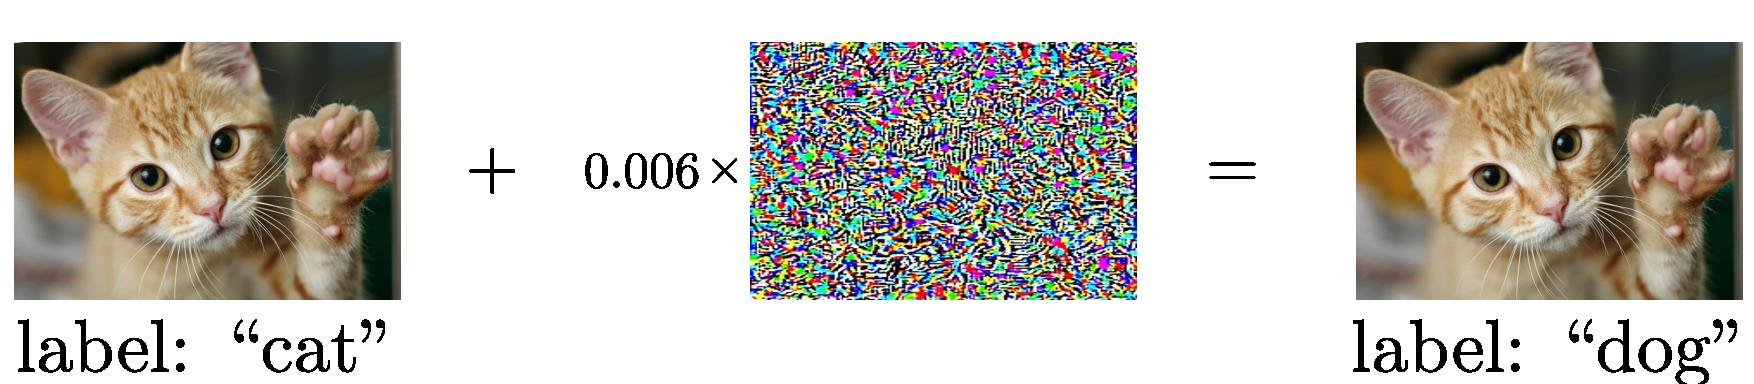
\includegraphics[width=\textwidth]{figures/main/ch1-introduction/ExampleAdversarialCatDog.pdf}
  \caption{Example of Adversarial Attack on an image.}
  \label{figure:ch1-adversarial_image_example}
\end{figure}

An example of widely used neural networks with specialized and more compact linear operations are \emph{Convolutional Neural Networks} (CNN)~\cite{lecun1998gradient,krizhevsky2012imagenet,he2016deep,tan2019efficientnet} which achieve state-of-the-art results for computer vision tasks.
Convolutional neural networks use specific weight matrices which encode the translation invariant property often desirable to process images.
% They use convolutional layers which are specific to image processing and use very few parameters.
Whereas a classical linear layer with a dense matrix will have $n \times n$ parameters, a convolution layer only has $k \times k$ parameters where $k \ll n$ is the kernel size and is usually small (\eg, 3 or 5 for classical convolutional layers).
A convolutional neural network is the most common type of \emph{structured} neural network.
Indeed, the convolution operation can be represented by a structured matrix \ie, a matrix that can be represented with less than $n^2$ parameters.


In addition to offering a more compact representation, the structure of certain matrices can be exploited to obtain better algorithms for the matrix-vector product, thus optimizing memory and computing operations.
Based on the success of convolutional neural networks, researchers have studied and proposed other types of neural networks based on weight matrices with different structures~\cite{moczulski2016acdc,sindhwani2015structured}.
\Cref{figure:ch1-example_structure_matrices} shows different types of structured matrices that have been used for deep learning.
Although convolutional neural networks have been state-of-the-art for computer vision tasks, it remains unclear whether other types of structured neural networks can be beneficial to other types of applications and which type of structure can provide both accuracy and efficient computation.

The contributions of this thesis lie at the intersection of linear algebra, Fourier analysis and deep learning.
As a result, we build compact and secure neural networks by leveraging the properties of structured matrices from the Toeplitz family.
Hereafter, we detail our contributions.

%%%%%%%%%%%%%%%%%%%%%%%%%%%%%%%%%%%%%%%%%%%%%%%%%%%%%%%%%%%%%%%%%%%%%%%%%%%%%%%%
\subsection{Training Compact Neural Networks}
\label{subsection:ch1-training_compact_neural_networks}
%%%%%%%%%%%%%%%%%%%%%%%%%%%%%%%%%%%%%%%%%%%%%%%%%%%%%%%%%%%%%%%%%%%%%%%%%%%%%%%%


% In addition, neural networks with a smaller number of parameters generalize better.
% This phenomenon has been theoretically justified by \citet{vapnik1982estimation}.
% Indeed, \citeauthor{vapnik1982estimation} linked the generalization capability of neural networks to their VC-dimension which is a measure of expressivity of the class of functions.
% This complexity measure is based on the number of parameters, therefore, reducing the number of parameters leads to a smaller VC-Dimension, which then leads to better generalization.

As a first contribution, we use circulant matrices, which are a particular type of Toeplitz matrix, to devise a new compact architecture replacing fully connected neural networks.
More precisely, we study deep diagonal-circulant neural networks, which are deep neural networks in which weight matrices are the product of diagonal and circulant ones.
Besides making a theoretical analysis of their expressivity, we introduce principled techniques for training these models: we devise an initialization scheme and propose a smart use of nonlinearity functions in order to train deep diagonal circulant networks.
Furthermore, we show that these networks outperform recently introduced deep networks with other types of structured layers.
We conduct a thorough experimental study to compare the performance of deep diagonal circulant networks with state-of-the-art models. 
%based on structured matrices and with dense models.
We show that our models achieve better accuracy than other structured approaches while requiring 2x fewer weights than the next best approach.
Finally, we train accurate deep diagonal circulant networks on a real-world video classification dataset with over 3.8 million training examples.
% Finally, we train deep diagonal circulant networks on a real-world video classification dataset with over 3.8 million training examples.

The training procedure we have developed to train large diagonal-circulant neural networks was first published in the \textbf{\color{mydarkblue} European Conference on Computer Vision Workshops on Video Classification}, as part of the \yt challenge.
Then, the theoretical analysis of the expressivity of diagonal-circulant neural networks has been published in a second paper in the \textbf{\color{mydarkblue} 24th European Conference on Artificial Intelligence}.



%%%%%%%%%%%%%%%%%%%%%%%%%%%%%%%%%%%%%%%%%%%%%%%%%%%%%%%%%%%%%%%%%%%%%%%%%%%%%%%%
\subsection{Training Robust Neural Networks}
\label{subsection:ch1-training_robust_neural_networks}
%%%%%%%%%%%%%%%%%%%%%%%%%%%%%%%%%%%%%%%%%%%%%%%%%%%%%%%%%%%%%%%%%%%%%%%%%%%%%%%%

As a second contribution, we build robust neural networks by studying the properties of the structure of convolutions.
We devise a new upper bound on the largest singular value of convolution layers that is both tight and easy to compute.
Our work is based on the result of~\citet{gray2006toeplitz} which states that an upper bound on the singular value of Toeplitz matrices can be computed from the inverse Fourier transform of the characteristic sequence of these matrices.
From our analysis immediately follows an algorithm for bounding the Lipschitz constant of a convolutional layer, and by extension the Lipschitz constant of the whole network.
Finally, we illustrate our approach to adversarial robustness.
Recent work has shown that empirical methods such as adversarial training offer poor generalization~\cite{schmidt2018adversarially} and can be improved by applying Lipschitz regularization~\cite{farnia2018generalizable}.
To illustrate the benefit of our new method, we train neural networks with Lipschitz regularization and show that it offers a significant improvement over adversarial training alone.

The main result of the work described in \Cref{chapter:ch5-lipschitz_bound} has been published in the \textbf{\color{mydarkblue}\nth{35} AAAI Conference on Artificial Intelligence}.
Additional joint contributions have also been published on the topic of robust neural networks.
The first work, published in the \textbf{\color{mydarkblue} Advances in Neural Information Processing Systems}, studies the effectiveness of noise injection at training and inference time in the network to protect against adversarial attacks.
In this work, we show that noise drawn from the Exponential family offers a provable protection against adversarial attacks. 
The second joint contribution published in the \textbf{\color{mydarkblue} European Conference on Machine Learning Workshop for CyberSecurity}, conducts a geometrical analysis of defense mechanisms designed to protect neural networks against several types of attacks.
This work shows that neural networks designed to be robust against one type of adversarial example offer poor against other types of attacks.





% In this thesis, we study the properties of structured matrices from the Toeplitz family and make contributions to the field of supervised learning with neural networks.
% This thesis is organized in two parts.
% First, we use circulant matrices, which are a particular case of Toeplitz matrices, to devise a new compact architecture replacing Fully Connected Neural Networks.
% More precisely, we study deep diagonal-circulant neural networks, which are deep neural networks in which weight matrices are the product of diagonal and circulant ones.
% Besides making a theoretical analysis of their expressivity, we introduce principled techniques for training these models: we devise an initialization scheme and propose a smart use of nonlinearity functions in order to train deep diagonal circulant networks.
% Furthermore, we show that these networks outperform recently introduced deep networks with other types of structured layers.
% We conduct a thorough experimental study to compare the performance of deep diagonal circulant networks with state-of-the-art models based on structured matrices and with dense models.
% We show that our models achieve better accuracy than other structured approaches while requiring 2x fewer weights than the next best approach.
% Finally, we train compact and accurate deep diagonal circulant networks on a real-world video classification dataset with over 3.8 million training examples.
% In the second part of this thesis, we study the properties of the structure of convolution to devise a new upper bound on the largest singular value of convolution layers that is both tight and easy to compute.
% Our work is based on the result of~\citet{gray2006toeplitz} which states that an upper bound on the singular value of Toeplitz matrices can be computed from the inverse Fourier transform of the characteristic sequence of these matrices.
% From our analysis immediately follows an algorithm for bounding the Lipschitz constant of a convolutional layer, and by extension the Lipschitz constant of the whole network.
% Finally, we illustrate our approach on adversarial robustness.
% Recent work has shown that empirical methods such as adversarial training (AT) offer poor generalization~\cite{schmidt2018adversarially}, and can be improved by applying Lipschitz regularization~\cite{farnia2018generalizable}.
% To illustrate the benefit of our new method, we train neural networks with Lipschitz regularization and show that it offers a significant improvement over adversarial training alone.


%%%%%%%%%%%%%%%%%%%%%%%%%%%%%%%%%%%%%%%%%%%%%%%%%%%%%%%%%%%%%%%%%%%%%%%%%%%%%%%
\section*{Outline of the Thesis}
\label{section:ch1-outline_of_the_thesis}
%%%%%%%%%%%%%%%%%%%%%%%%%%%%%%%%%%%%%%%%%%%%%%%%%%%%%%%%%%%%%%%%%%%%%%%%%%%%%%%

This thesis is organized in six chapters.
First, \Cref{chapter:ch2-background} gives an introduction to the theory of Toeplitz matrices and on supervised learning and neural networks.
This chapter presents the necessary technical tools we will need for presenting the related work and for our contributions.
\Cref{chapter:ch3-related_work} is dedicated to enumerating the state-of-the-art approaches.
The chapter is divided into two parts.
First, we review techniques to build compact neural networks with an important focus on techniques that use structured matrices.
The second part focuses on presenting regularization methods for improving the robustness of neural networks.
\Cref{chapter:ch4-diagonal_circulant_neural_network} and \Cref{chapter:ch5-lipschitz_bound} constitute our main contributions.
\Cref{chapter:ch4-diagonal_circulant_neural_network} presents results on compact neural networks built from diagonal and circulant matrices.
\Cref{chapter:ch5-lipschitz_bound} presents our new regularization scheme to improve the robustness of neural networks based on the properties of doubly-block Toeplitz matrices.
\Cref{chapter:ch6-conclusion} proposed a discussion and some perspectives on the contributions.
Appendix~\ref{appendix:ap2-diagonal_circulant_neural_networks_for_video_classification} constitutes some complements to~\Cref{chapter:ch4-diagonal_circulant_neural_network}.
It provides additional experiments on video classification with compact neural networks.
Finally, Appendix~\ref{appendix:ap3-theoretical_evidence_for_adversarial_robustness_through_randomization} and Appendix~\ref{appendix:ap4-advocating_multiple_defense_strategies_against_adversarial_examples} provide further work on the robustness of neural networks done during this Ph.D. thesis.
% Finally, Appendix~\ref{appendix:ap6-publications} enumerates the publications made during this Ph.D. thesis.




